\documentclass[svgnames]{beamer}

\usetheme{Madrid}
\usecolortheme{seahorse}
\usepackage{multirow}
\usepackage{caption}
\setbeamertemplate{navigation symbols}{}
\useinnertheme{rectangles}
\usepackage{varwidth}
\usepackage{xparse}
\usepackage{appendixnumberbeamer}
\usepackage[ruled, vlined, longend]{algorithm2e}
\beamertemplatenavigationsymbolsempty
\usepackage[many]{tcolorbox}
\usetikzlibrary{decorations.pathmorphing}
\usetikzlibrary{fadings,shapes.arrows,shadows,shapes.callouts}   
\usepackage[absolute,overlay]{textpos}
\usepackage{listings}
\lstset {
  backgroundcolor=\color{white},
  basicstyle=\ttfamily\footnotesize,
  numbers=left,numberstyle=\tiny,numbersep=5pt,
  emph={proc, fun, let, send, consume, global, type, record, if, else,
    in, not, foldt, return, on, ordering, by, as, or },
  emphstyle={\bfseries},
  literate = {=>}{{\bf=>}}2
}
\usepackage{graphicx,accents,pinlabel}

\definecolor{paper}{RGB}{239,227,157}
\newtcolorbox{tornpage}{%
    enhanced jigsaw, breakable, % allow page breaks
    frame hidden, % hide the default frame
    overlay={%
        \draw [
            fill=paper, % fill paper
            draw=paper!50!black, % boundary colour
            decorate, % decoration
            decoration={random steps,segment length=2pt,amplitude=1pt},
            drop shadow, % shadow
        ]
        % top line
        (frame.north west)--(frame.north east)--
        % right line
        (frame.north east)--(frame.south east)--
        % bottom line
        (frame.south east)--(frame.south west)--
        % left line
        (frame.south west)--(frame.north west);
    },
    % paragraph skips obeyed within tcolorbox
    parbox=false,
}
%\useoutertheme{default}
%\useinnertheme{rounded}

\titlegraphic{
\begin{center}
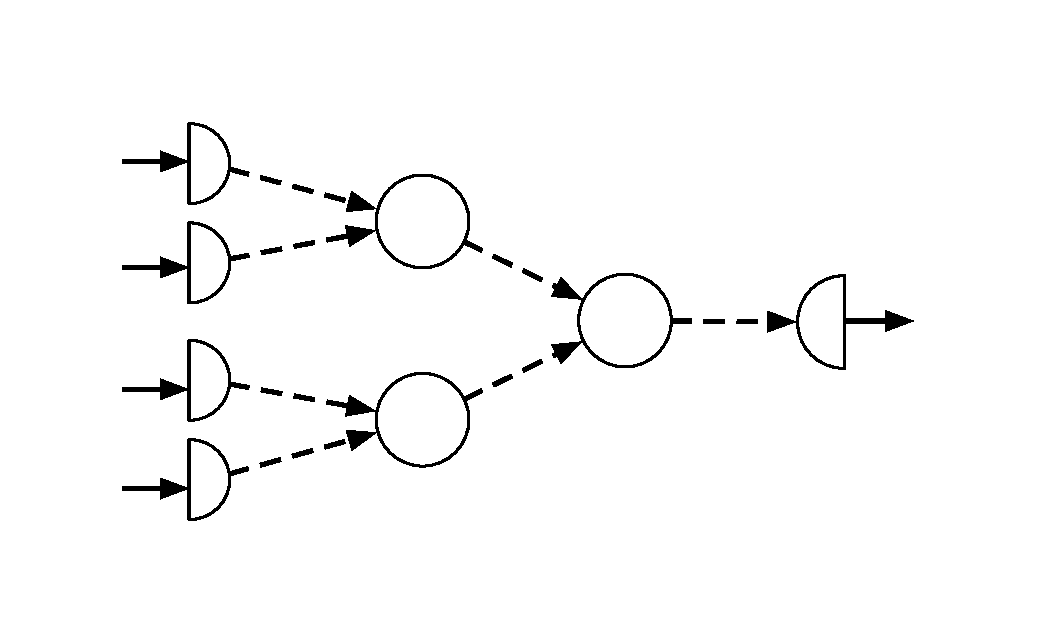
\includegraphics[width=3cm]{hadoop2}%
\end{center}
}

\usepackage{tikz}
\usetikzlibrary{shadows.blur}
\usetikzlibrary{shapes.symbols}
\usetikzlibrary{backgrounds}
\usetikzlibrary{arrows.meta}
\usetikzlibrary{shapes,snakes}
\usetikzlibrary{fit,calc,shadows}
\setbeamercolor{section in head/foot}{bg=white, fg=black}
%\beamertemplateshadingbackground{black!10}{blue!15}
\makeatletter
\setbeamertemplate{footline}
{
  \leavevmode%
  \hbox{%
  \begin{beamercolorbox}[wd=.333333\paperwidth,ht=2.25ex,dp=1ex,center]{section in head/foot}%
    \usebeamerfont{author in head/foot}\insertshortauthor~~\beamer@ifempty{\insertshortinstitute}{}{Richard G. Clegg}
  \end{beamercolorbox}%
  \begin{beamercolorbox}[wd=.333333\paperwidth,ht=2.25ex,dp=1ex,center]{section in head/foot}%
    \usebeamerfont{title in head/foot}{Studying Gab with Raphtory}
  \end{beamercolorbox}%
  \begin{beamercolorbox}[wd=.333333\paperwidth,ht=2.25ex,dp=1ex,right]{section in head/foot}%
    \usebeamerfont{date in head/foot}\insertshortdate{}\hspace*{2em}
    \insertframenumber{} / \inserttotalframenumber\hspace*{2ex} 
  \end{beamercolorbox}}%
  \vskip0pt%
}
\makeatother

\date[QMUL IADS]{Presentation to QMUL IADS}

\begin{document}


\frame{

\title[Raphtory]{A new tool for large temporal networks applied to the far right social network Gab}

\setcounter{framenumber}{0}

\begin{center}
\Huge{Raphtory: A new tool for large temporal networks applied to the far right social network Gab}


\vspace{0.2cm}

\inserttitlegraphic

\vspace{0.2cm}

\scriptsize{\raggedright
{\color{blue} Presenter: }Richard G. Clegg,  \\}
\scriptsize{\raggedright
%Work joint with the {\color{blue} Network-as-a-Service project}.  \\
{
    {\color{blue} Project team (alphabetical order): \\ }
Naomi Arnold, F\'{e}lix Cuadrado, Imane Hafnaoui, Raul Mondragon, Hugo Parada, Ben Steer }
}

%\tiny{(Prepared using \LaTeX \;and beamer.)}
\end{center}
}

\tikzset{onslide/.code args={<#1>#2}{%
  \only<#1>{\pgfkeysalso{#2}} % \pgfkeysalso doesn't change the path
}}
\tikzset{temporal/.code args={<#1>#2#3#4}{%
  \temporal<#1>{\pgfkeysalso{#2}}{\pgfkeysalso{#3}}{\pgfkeysalso{#4}} % \pgfkeysalso doesn't change the path
}}

\tikzstyle{platform} = [draw=black,shade, 
      anchor=south west,
      align= center,
      top color=blue!40,
      bottom color=blue!5,
      rounded corners=6pt,
      blur shadow={shadow blur steps=5},
      font = \footnotesize]

\section{Introduction}


\tikzstyle{box} = [draw=black,shade, 
      font = \footnotesize,
      align= center,
      top color=blue!40,
      bottom color=blue!5,
      rounded corners=3pt,
      blur shadow={shadow blur steps=5}]

\tikzstyle{box2} = [draw=black,shade, 
      font = \footnotesize,
      align= center,
      top color=red!40,
      bottom color=red!5,
      rounded corners=3pt,
      blur shadow={shadow blur steps=5}]

\tikzstyle{net con} = [draw=black,ultra thick]

\frame{
    
    \frametitle{Aims of this talk (unordered list)}

\begin{block}{Aim A: Give insight into data}
What drives the evolution of the alt-right social network gab?
\end{block}
\pause
\begin{block}{Aim 1: Show a technique}
Temporal analysis and in particular ``windowing" is an invaluable tool for social network analysis. 
\end{block}
\pause
\begin{block}{Aim $\alpha$: Sell you a tool}
Raphtory is an open-source, big-data platform developed at QMUL. It is unique in its ability to perform flexible temporal analysis on batch or streamed graph data.
\end{block}
    
}

\frame{
    \frametitle{The gab platform (and why we care)}
\centering{
\begin{tikzpicture}%[show background grid]
\draw[white] (-5.5,-3.5) rectangle (5.5,3.5);
\node <1-> at (0,0) {
    {\begin{varwidth}{\linewidth}
\begin{itemize}
\item 95GB raw data (19 million posts) from gab platform (\alert{medium} data).
\begin{itemize}
\item Data is user, posts (threaded), timestamps and other metadata.
\item NB our research on \alert{structure} not \alert{content}.
\end{itemize} 
\item First eighteen months of data available. 
\begin{itemize}
\item September 2016 -- May 2018.
\end{itemize}
\item Largely complete data from this period.
\begin{itemize} 
\item``free speech" focus means ``everything" is public.
\end{itemize}
\item Alt-right focus: 
\begin{itemize}
\item Racism, fake news, hate speech, radicalisation.
\end{itemize}
\end{itemize}
\end{varwidth}}
};
\node <2-> at (-2,0) {
\includegraphics[width=7cm,angle=20]{gab1}};
\node <3-> at (2,2) {
\includegraphics[width=8cm,angle=-10]{gab2}};
\node <4-> at (-1,0) {
\includegraphics[width=8cm,angle=-30]{gab3}};
\node <5-> at (0,0) {
\includegraphics[width=6cm,angle=40]{gab4}};
\end{tikzpicture}
}


}

\tikzfading[name=arrowfading, top color=transparent!0, bottom color=transparent!95]
\tikzset{arrowfill/.style={#1,general shadow={fill=black, shadow yshift=-0.8ex, path fading=arrowfading}}}
\tikzset{arrowstyle/.style n args={3}{draw=#2,arrowfill={#3}, single arrow,minimum height=#1, single arrow,
single arrow head extend=.3cm,}}

\NewDocumentCommand{\tikzfancyarrow}{O{2cm} O{FireBrick} O{top color=OrangeRed!20, bottom color=Red} m}{
\tikz[baseline=-0.5ex]\node [arrowstyle={#1}{#2}{#3}] {#4};
}




\frame{
    \frametitle{The Raphtory tool}
\begin{tikzpicture}%[show background grid]
\draw[white] (-5.5,-3.5) rectangle (5.5,3.5);
\node <1-> at (-4.5,0) {
\includegraphics[width=1.5cm]{tweet}};
\node <1-> at (-0.5,-2) {
\includegraphics[width=2cm]{computer}};
\node <1-> at (-0.5,2) {
\includegraphics[width=2cm]{computer}};
\node <1-> at (2.5,2) {
\includegraphics[width=2cm]{computer}};
\node <1-> at (2.5,-2) {
\includegraphics[width=2cm]{computer}};
\node <1-> at (5.5,0) {
\includegraphics[width=1.2cm]{user}};
\node <2-> at (-2.5,0) {\tikzfancyarrow[1.5cm][DarkBlue][top color= PaleTurquoise,bottom color=DeepSkyBlue]{link data} };
\node <2-> at (-2.5,0) {\tikzfancyarrow[1.5cm][DarkBlue][top color= PaleTurquoise,bottom color=DeepSkyBlue]{link data} };
\node <2-> at (-2.5,-1.2) {\tikzfancyarrow[1.5cm][DarkBlue][top color= PaleTurquoise,bottom color=DeepSkyBlue]{link data} };
\node <2-> at (-2.5,1.2) {\tikzfancyarrow[1.5cm][DarkBlue][top color= PaleTurquoise,bottom color=DeepSkyBlue]{link data} };
\node <3> at (1,0) {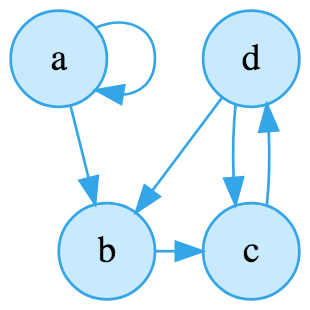
\includegraphics[width=2cm]{graphfull}};
\node <4-> at (-0.5,-2) {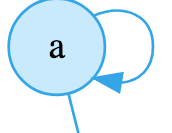
\includegraphics[width=1cm]{grapha}};
\node <4-> at (-0.5,2) {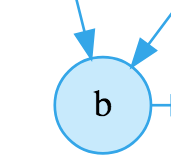
\includegraphics[width=1cm]{graphb}};
\node <4-> at (2.5,2) {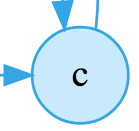
\includegraphics[width=1cm]{graphc}};
\node <4-> at (2.5,-2) {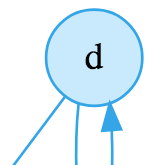
\includegraphics[width=1cm]{graphd}};
\node <5-> at (3.7,0) {\tikzfancyarrow[2.5cm][Orchid][top color= Thistle,bottom color=Orchid,shape border rotate=180]{user query} };
\node<6->[platform,anchor= north] at (0,2) {What does the graph look like now?};
\node<7->[platform,anchor= north] at (0,1.) {What did the graph look like last week?};
\node<8->[platform,anchor= north] at (0,0) {How does the graph change each month/day/second?};
\node<9->[platform,anchor= north] at (0,-1) {What time did the graph change most?};
\node<10->[platform,anchor= north] at (0,-2) {How did the graph change when user $u$ arrived?};
\end{tikzpicture}
}

\frame{
    \frametitle{Social network analysis}
\begin{block}{Social network $\rightarrow$ graph $G$ }
We can form a graph from a social network by creating an edge between two users if they are friends or if they ``mention" each other. 
\end{block}
\pause
\begin{block}{Social network $\rightarrow$ many graphs $G(t,\tau)$}
There is no such thing as \alert{``the twitter graph"}. The graph varies hugely depending on the \alert{time} and \alert{timescale}.
\end{block}
}

\frame{
    \frametitle{Temporal graphs -- interaction graphs}
\begin{block}{Interaction graph for time $t$ and a window length $\tau$}
The graph $G(t,\tau)$ is defined by the set of all edges $i,j$ where $i$ and $j$ interact at a time $T$ such that $t-\tau/2 \leq T \leq t + \tau/2$.
\end{block}
\centering{
\begin{tikzpicture}%[show background grid]
\node<1-> at (0,0){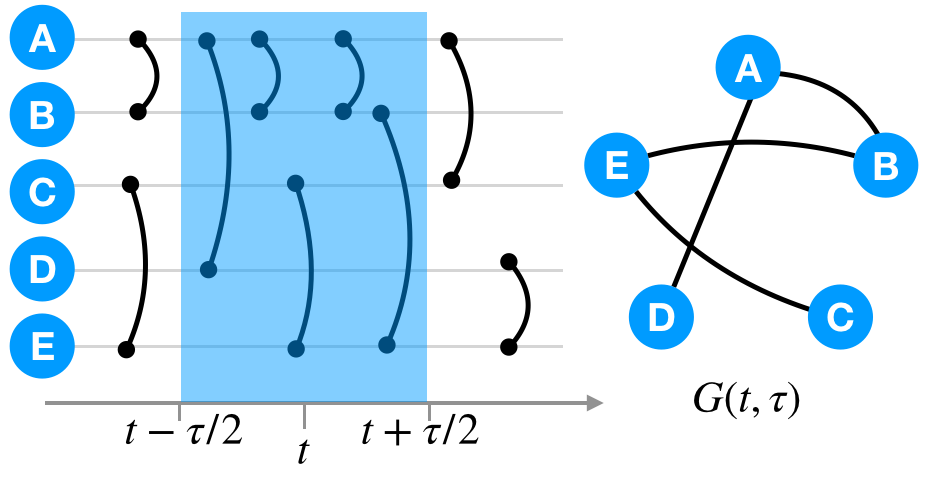
\includegraphics[width=0.8\textwidth]{windowing_schematic}};
\node<2-> at (0,0) [platform,anchor= south] {Intuition: Increasing $\tau$ will add nodes and density};
\node<3-> at (0,-1) [platform,anchor= south] {Intuition: Decreasing $\tau$ will reduce nodes and density};
\end{tikzpicture}
}
}

\frame{
\frametitle{Checking our intuition}
\centering{
\begin{tikzpicture}%[show background grid]
\node<1> at (0,0){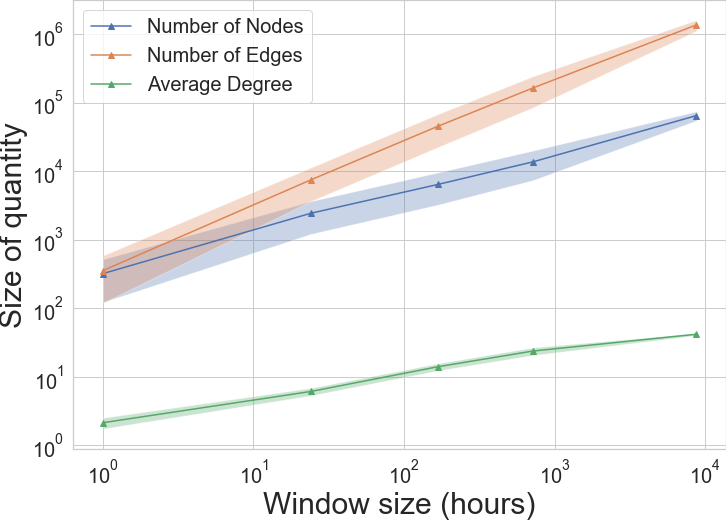
\includegraphics[width=0.8\textwidth]{windowscale}};
\end{tikzpicture}
}
}

\section{Analysis}

\tikzstyle{cloudconn} = [draw=black, inner sep=0pt,
       line width=0.25mm,{Latex[length=2.5mm, width=1.5mm]}-{Latex[length=2.5mm, width=1.5mm]}]

\tikzstyle{arrowconn} = [draw=black, inner sep=0pt,
       line width=0.25mm,-{Latex[length=2.5mm, width=1.5mm]}]

\frame{
\frametitle{What drives growth on gab?}
\centering{
\begin{tikzpicture}%[show background grid]
\node<1-> at (0,0){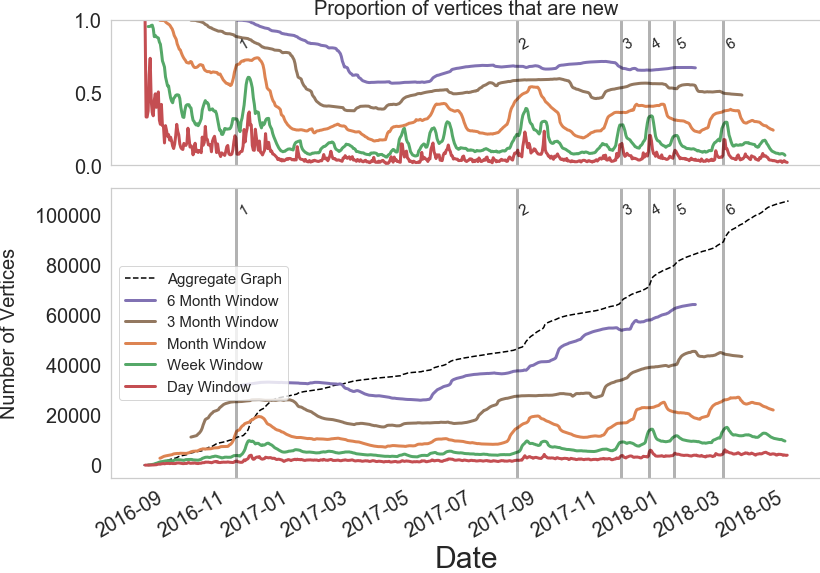
\includegraphics[width=0.8\textwidth]{vertices}};
\node<2> at (0,0) [platform,anchor= south] (e1) {09/11/16 -- Trump wins election};
\node<3> at (0,0) [platform,anchor= south] (e2) {11/08/17 -- Unite the Right rally};
\node<4> at (0,0) [platform,anchor= south] (e3) {21/11/17 -- Plan to repeal neutrality announced};
\node<5> at (0,0) [platform,anchor= south] (e4) {18/12/17 -- Twitter suspends white nationalists};
\node<6> at (0,0) [platform,anchor= south] (e5) {12/01/18 -- Trump `sh*thole countries' comment};
\node<7> at (0,0) [platform,anchor= south] (e6) {01/03/18 -- Gilmore lawsuit against Alex Jones};
\node at (-2.2,2.0) (e1p) {};
\node at (1.3,2.0) (e2p) {};
\node at (2.5,2.0) (e3p) {};
\node at (2.9,2.0) (e4p) {};
\node at (3.2,2.0) (e5p) {};
\node at (3.8,2.0) (e6p) {};
\path[draw] <2> (e1) edge[arrowconn] (e1p);
\path[draw] <3> (e2) edge[arrowconn] (e2p);
\path[draw] <4> (e3) edge[arrowconn] (e3p);
\path[draw] <5> (e4) edge[arrowconn] (e4p);
\path[draw] <6> (e5) edge[arrowconn] (e5p);
\path[draw] <7> (e6) edge[arrowconn] (e6p);
\end{tikzpicture}
}
}



\frame{
\frametitle{Is gab a ``social" network?}
\centering{
\begin{tikzpicture}%[show background grid]
\node<1> at (0,0){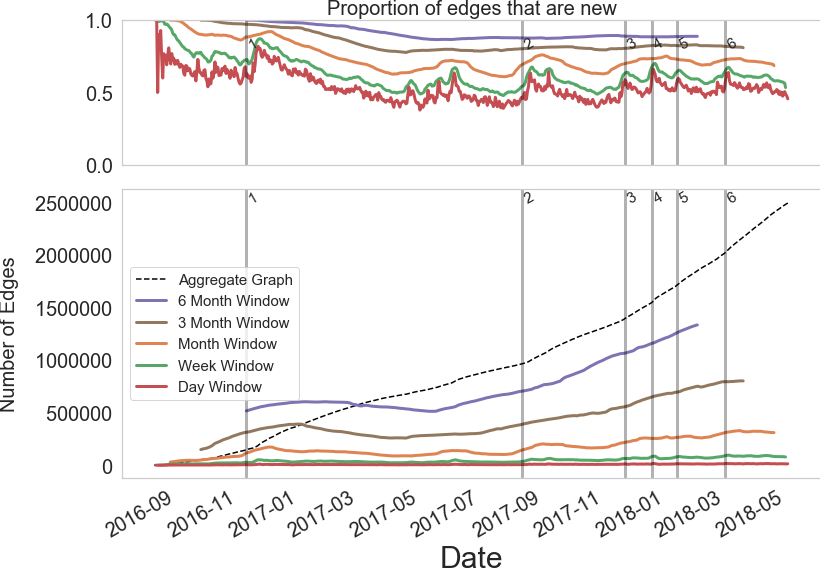
\includegraphics[width=0.8\textwidth]{edges}};
\end{tikzpicture}
}
}

\frame{
\frametitle{Is gab a community?  Largest Connected Component}

\begin{block}{Definition:Connected component}
A \alert{connected component} is a sub graph of a graph within which all nodes can trace a path to each other.
The largest connected component (LCC) is the one with the most nodes.
\end{block}
\pause
\begin{itemize}
\item In a typical social network we can trace a path between most node pairs.
\item Rare sets of nodes interact only with each other. 
\item LCC is size of the largest ``community" (in loosest sense).
\item Sub graphs outside LCC have no connection at all with LCC.
\item Remember: only count people active within the window.
\item Expectation: in a ``large" window most users within the LCC.
\item But what happens as we look at smaller and smaller windows?
\end{itemize}
}

\frame{
\frametitle{Is gab a community?  Largest Connected Component}
\centering{
\begin{tikzpicture}%[show background grid]
\node<1> at (0,0){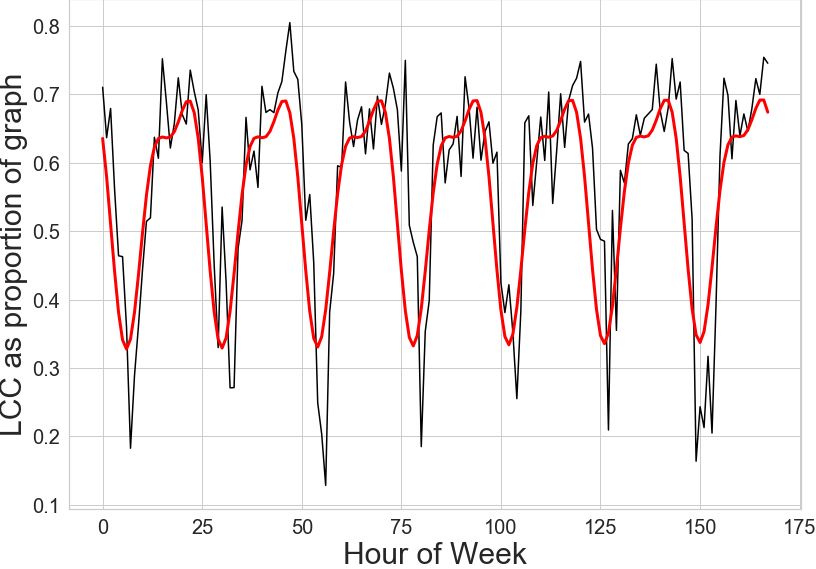
\includegraphics[width=0.8\textwidth]{lcc}};
\end{tikzpicture}
}
}

%\frame{
%\frametitle{Is gab a community?  Largest Connected Component}
%\centering{
%\begin{tikzpicture}%[show background grid]
%\node<1> at (0,0){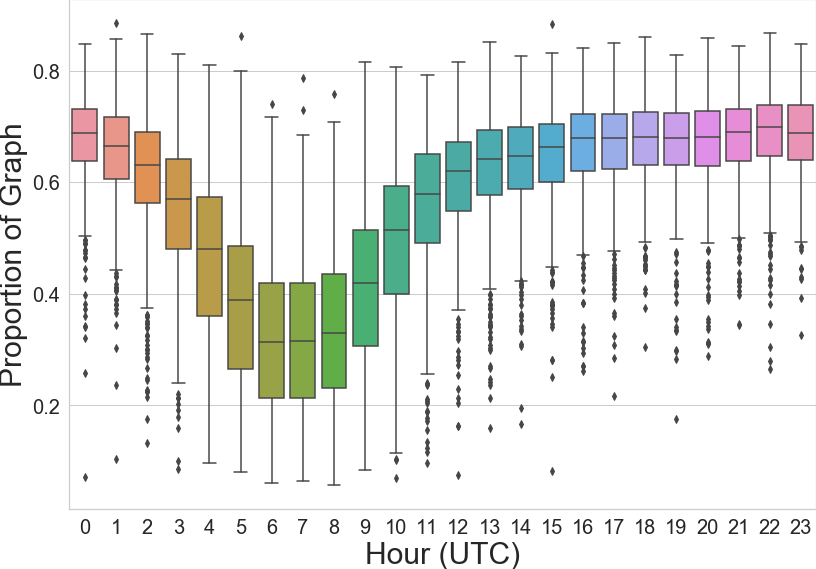
\includegraphics[width=0.8\textwidth]{prop_diurnal}};
%\end{tikzpicture}
%}
%}

      

\frame{
    \frametitle{Is gab controlled by an ``elite"?}
\begin{itemize}
\item One measurement: Are the same people always most ``talked about"?
\item Proxy measurement: Node degree is the number of users who engaged with that user.
\item Are highest degree nodes same between windows $W_A$ and $W_B$?
\end{itemize}
\pause
\begin{block}{Jaccard Similarity (for top $N$ users)}
Let $A,B$ be set of top $N$ users in windows $W_A,W_B$.
$$J(A,B) = \frac{A \cap B}{A \cup B}.$$
\end{block}
\pause
\begin{block}{Refresh rate top $N$ users, windows $W_A$,$W_B$}
Refresh rate $R= 1-J(A,B)$ \\
$0 \rightarrow W_A$ same users as $W_B$ and $1 \rightarrow$ no users the same.
\end{block}
}

\frame{
    \frametitle{Is gab controlled by an ``elite"?}
\centering{
\begin{tikzpicture}%[show background grid]
\node<1> at (0,0){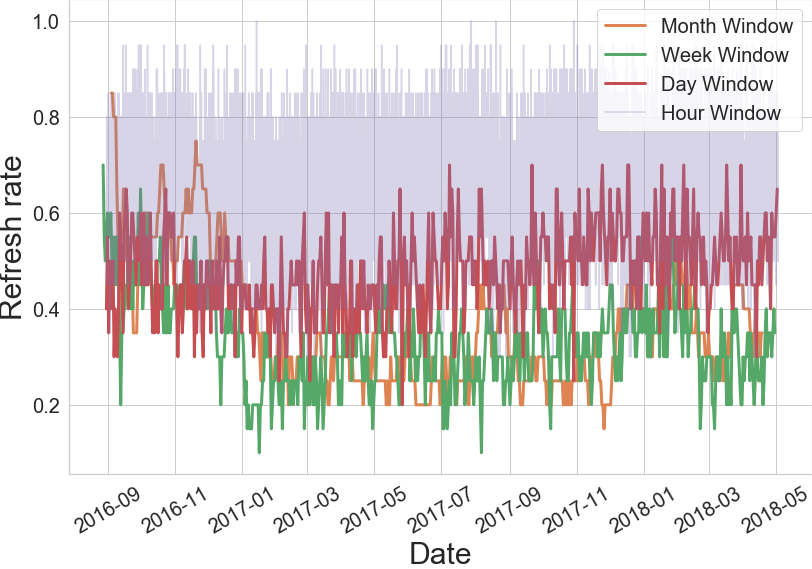
\includegraphics[width=0.8\textwidth]{jaccard}};
\end{tikzpicture}
}
}





\frame{
    \frametitle{Is gab controlled by an ``elite"?}
\centering{
\begin{tikzpicture}[->]%[show background grid]
\node<1-> at (0,0){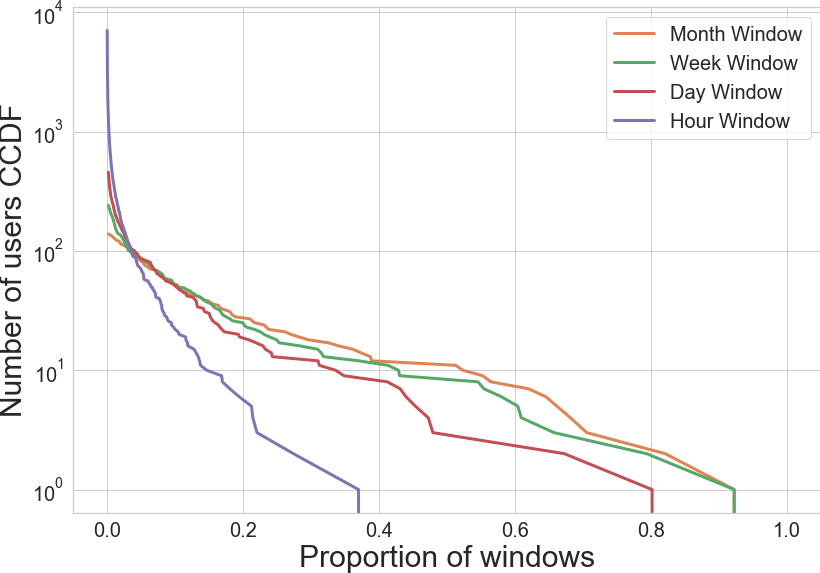
\includegraphics[width=0.8\textwidth]{top20CCDF}};
\node<2-> at (1,0) [platform,anchor= south] (monthwt) {Eleven users are in $> 50\%$ monthly windows};
\node<3-> at (-1,-1.7) [platform,anchor= south] (hourwt) {No users are in $> 40\%$ hourly windows};
\node at (0.4,-1.1) (monthw) {};
\node at (-0.5,-2.5) (hourw) {};
\path[draw] <2-> (monthwt) edge[arrowconn] (monthw);
\path[draw] <3-> (hourwt) edge[arrowconn] (hourw);
\end{tikzpicture}
}
}

\section{Conclusions}
\frame{
\frametitle{Conclusions (about gab)}    
\begin{itemize}
\item Is gab growing? What drives this?
\begin{itemize}
\item Long duration (months to years) gab is growing relatively slowly.
\item Short duration (hours to days) we can witness rapid growth.
\item Growth driven by community specific events.
\end{itemize}
\pause
\item Gab is not a ``social" network -- interactions between ``strangers" not friends.
\pause
\item Analysed at the hourly level not always a ``connected" community
\begin{itemize}
\item Graph LCC shatters into disconnected pieces at off-peak hours.
\item This diurnal change of regime never observed before.
\end{itemize}
\pause
\item Are a cadre of elite users controlling users' attention? 
\begin{itemize}
\item Not clear: At longer timescales there are a group who have a lot of attention.
\item If you look at only one timescale you will get a misleading answer.
\end{itemize}
\end{itemize}
}
\frame{
\frametitle{Conclusions (about Raphtory and temporal networks)}    
\begin{itemize}
\item Temporal networks provide a rich array of techniques that can get more out of your network data.
\begin{itemize}
\item Window based analysis provides many levels of insight. 
\item Akin to looking at frequency as well as time.
\pause
\end{itemize}
\item Other Raphtory use cases we are working on:
\begin{itemize}
\item Urban analytics -- intervention in social networks.
\item Bitcoin/blockchain -- tracking ``dark markets".
\item Semantic networks -- changing word meanings.
\item Other social networks -- compare and learn more.
\pause
\end{itemize}
\item The Raphtory tool is a great way to look at temporal graph data.
\begin{itemize}
\item Funding from the Alan Turing Institute for development.
\item Spin off company Chorograph pushing adoption.
\item We can help you use it on your data sets.
\end{itemize}
\end{itemize}
}



\frame{
\frametitle{Our Raphtory social network (a small subgraph)}
\centering{
\begin{tikzpicture}%[show background grid]
\draw[white] (-5,-3) rectangle (5,3);
\node <1-> [inner sep=0pt] at (-4.5,0.0) (fc) {
\includegraphics[width=1.5cm]{felix}};
\node <1-> [inner sep=0pt] at (4.5,0.0) (ih) {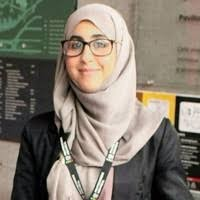
\includegraphics[width=1.5cm]{imane}};
\node <1-> [inner sep=0pt] at (-3,2.5) (bs) {
\includegraphics[width=1.5cm]{ben}};
\node <1-> [inner sep=0pt] at (3,2.5) (rc) {
\includegraphics[width=1.5cm]{rich}};
\node <1-> [inner sep=0pt] at (-3,-2.5) (rm) {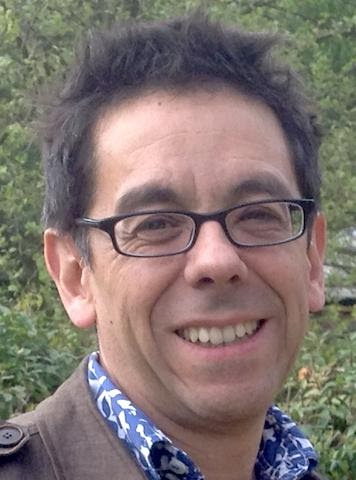
\includegraphics[width=1.5cm]{raul}};
\node <1-> [inner sep=0pt] at (3,-2.5) (na) {
\includegraphics[width=1.5cm]{naomi}};


\path[draw] <3-> (ih) edge[cloudconn] (fc);
\path[draw] <3-> (ih) edge[cloudconn] (bs);
\path[draw] <3-> (ih) edge[cloudconn] (rc);
\path[draw] <3-> (ih) edge[cloudconn] (na);
\path[draw] <3-> (ih) edge[cloudconn] (rm);
\path[draw] <2-> (fc) edge[cloudconn] (bs);
\path[draw] <2-> (fc) edge[cloudconn] (rc);
\path[draw] <2-> (fc) edge[cloudconn] (rm);
\path[draw] <2-> (fc) edge[cloudconn] (na);
\path[draw] <2-> (bs) edge[cloudconn] (rc);
\path[draw] <2-> (bs) edge[cloudconn] (na);
\path[draw] <2-> (bs) edge[cloudconn] (rm);
\path[draw] <2-> (na) edge[cloudconn] (rc);
\path[draw] <2-> (na) edge[cloudconn] (rm);
\path[draw] <2-> (rc) edge[cloudconn] (rm);
\node<4>[platform,anchor= south] at (0,0.1) {Paper on gab and temporal graphs \\
submitted to ICWSM 2020 (under review)
};
\node<4>[platform,anchor= north] at (0,-0.1) {Raphtory is on github \\https://github.com/miratepuffin/raphtory
};
\end{tikzpicture}
}
}
\end{document}
